\section{Wrap-up}

\section*{ÜBERSICHT}
\begin{itemize}
  \item Von SuiWeb zu React.js
  \item Ausblick: Weitere Themen rund ums Web
  \item Abschluss, Feedback
  \item Anhang: Themenliste WBE
\end{itemize}

\section*{ÜBERSICHT}
\begin{itemize}
  \item Von SuiWeb zu React.js
  \item Ausblick: Weitere Themen rund ums Web
  \item Abschluss, Feedback
  \item Anhang: Themenliste WBE
\end{itemize}

\section*{SUIWEB}
\begin{itemize}
  \item SuiWeb ist eine experimentelle Bibliothek
  \item Angelehnt an die Ideen von React.js
  \item Es ist Zeit, React.js noch etwas anzusehen
\end{itemize}

\section*{REACT}
„A JavaScript library for building user interfaces"

\begin{itemize}
  \item Declarative
  \item Component-Based
  \item Learn Once, Write Anywhere
\end{itemize}

Facebook, Instagram\\
2013 vorgestellt\\
\href{https://react.dev}{https://react.dev}

\section*{ZWEI TEILE}
\begin{itemize}
  \item React DOM
  \item Performs the actual rendering on a web page\\
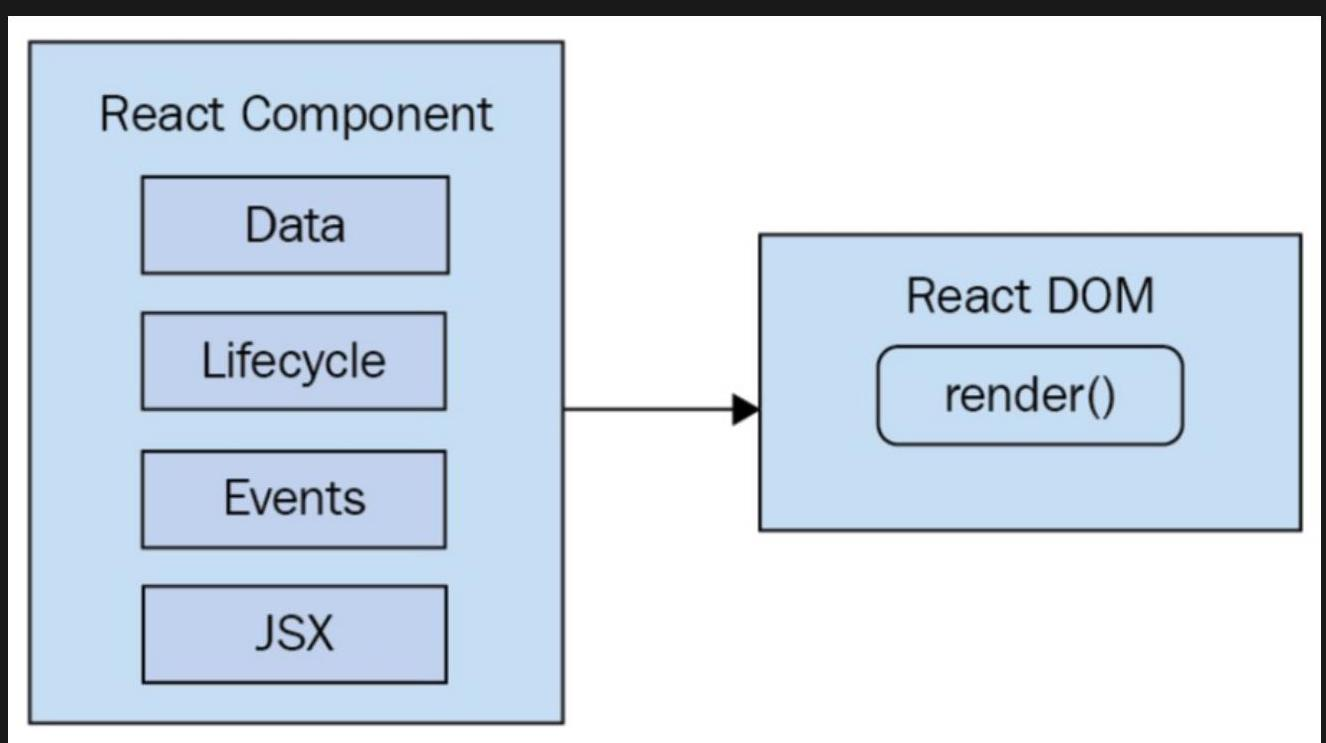
\includegraphics[width=\linewidth]{images/2025_01_02_68113d8fd21152cab1dbg-06}
  \item React Component API
  \item Data to be rendered
  \item Lifecycle methods
  \item Events: respond to user interactions
  \item JSX: syntax used to describe UI structures
\end{itemize}

\section*{KOMPONENTEN UND KLASSEN}
\begin{verbatim}
// ES5
var HelloComponent = React.createClass({
    render: function() {
        return <div>Hello {this.props.name}</div>
    }
})
// ES6
class HelloComponent extends React.Component {
    render() {
        return <div>Hello {this.props.name}</div>
    }
}
// Function Component
const HelloComponent = (props) => {
    return (<div>Hello {props.name}</div>)
}
\end{verbatim}

\section*{KOMPONENTEN}
\begin{verbatim}
const MyComponent = () => (
    <section>
        <h1>My Component</h1>
        <List data={["Maria", "Hans", "Eva", "Peter"]} />
    </section>
)
const List = ({data}) => (
    <ul>
        { data.map(item => (<li key={item}>{item}</li>)) }
    </ul>
)
const root = createRoot(document.getElementById('app'))
root.render(
    <MyComponent />
)
\end{verbatim}

\section*{ZUSTAND}
\begin{verbatim}
const Counter = () => {
    const [state, setState] = useState(1)
    const handler = () => setState(c => c + 1)
    return (
        <h1 onclick={handler} style={{userSelect:"none",cursor:"pointer"}}>
            Count {state}
        </h1>
    )
}
const root = createRoot(document.getElementById('counter'))
root.render(
    <Counter />
)
\end{verbatim}

\section*{PROPERTIES}
\begin{verbatim}
const MyButton = (props) => {
    const { disabled, text } = props
    return (
            <button disabled={disabled}>{text}</button>
    )
}
const root = createRoot(document.getElementById('counter'))
root.render(
    <main>
        <MyButton text='My Button' disabled=true />
    </main>
)
\end{verbatim}

\section*{UND SONST}
\begin{itemize}
  \item Funktions- und Klassenkomponenten unterstützt
  \item Funktionskomponenten mit Hooks (u.a. State Hook)
  \item Diverse Optimierungen: virtuelles DOM, Fibers
  \item Entwicklertools, React Devtools
  \item Serverseitiges und clienseitiges Rendern
  \item Komponententechnologie auch für native iOS und Android Apps verwendbar (React Native)
\end{itemize}

\section*{WAS IST NUN REACT?}
\begin{itemize}
  \item React bildet die View einer Applikation
  \item Nicht (nur) Framework, sondern in erster Linie Konzept
  \item Unterstützt das Organisieren von Vorlagen in Komponenten
  \item Das virtuelle DOM sorgt für schnelles Rendern
\end{itemize}

\section*{POWER OF COMPONENTS}
\begin{itemize}
  \item Kleinere Einheiten entwickeln
  \item Weniger Abhängigkeiten
  \item Einfacher zu verstehen, zu pflegen, zu testen
  \item Komponentendesign: für genau eine Sache verantwortlich
  \item Zustand in wenigen Komponenten konzentrieren
\end{itemize}

\section*{HAUPTKONZEPTE}
\begin{itemize}
  \item Klarer und einfacher Datenfluss:
  \item Daten nach unten weitergegeben (props)
  \item Ereignisse nach oben weitergegeben und dort behandelt
  \item Properties werden nicht geändert, Zustand ist veränderbar
  \item Zustand wird von Komponente verwaltet
  \item Es ist von Vorteil, die meisten Komponenten zustandslos zu konzipieren
\end{itemize}

\section*{Existing Frameworks Influenced: All of them}
\begin{itemize}
  \item Angular komplett überarbeitet
  \item Neue Frameworks entstanden: Vue.js, Svelte, ...
  \item Entwicklung nativer Mobil-Apps: SwiftUI, Compose
  \item ...
\end{itemize}

\section*{ÜBERSICHT}
\begin{itemize}
  \item Von SuiWeb zu React.js
  \item Ausblick: Weitere Themen rund ums Web
  \item Abschluss, Feedback
  \item Anhang: Themenliste WBE
\end{itemize}

\section*{HAUPTTHEMEN IN WBE}
\begin{itemize}
  \item JavaScript die Sprache (und Node.js)
  \item JavaScript im Browser
  \item Client-seitige Web-Apps
\end{itemize}

\section*{WEITERE THEMEN RUND UMS WEB}
Rund ums Web gibt es noch viele spannende Themen...\\
Ein paar Anregungen sind auf den folgenden Slides zusammengestellt (ohne Anspruch auf Vollständigkeit)

\section*{HTML und CSS}
\begin{itemize}
  \item Grundlagen: als Vorkenntnisse für WBE
  \item Skript im Vorbereitungskurs (Moodle)
  \item Diverse Tutorials (ein paar im Kurs verlinkt)\\
$\triangleright$ Vorbereitungskurs WBE
\end{itemize}

\section*{Web-Apps für Mobilgeräte}
\begin{itemize}
  \item Layout für verschiedene Devices (Smartphones, ...)
  \item Responsives Webdesign (u.a. Bilder)
  \item Web-APIs für Gerätesensoren
  \item Apps basierend auf React und Ionic
  \item React Native / Expo\\
$\triangleright$ MOBA
\end{itemize}

\section*{Mobile Applications (MOBA1/MOBA2)}
\begin{itemize}
  \item Mobile Layouts, CSS Flexbox
  \item Device APIs, Sensoren
  \item Web Components, React, Ionic
  \item React Native\\
und:
  \item Android native (Kotlin, Compose)
  \item iOS native (Swift, SwiftUI)
\end{itemize}

Info $\triangleright$ H. Stormer (stme), G. Burkert (bkrt)\\
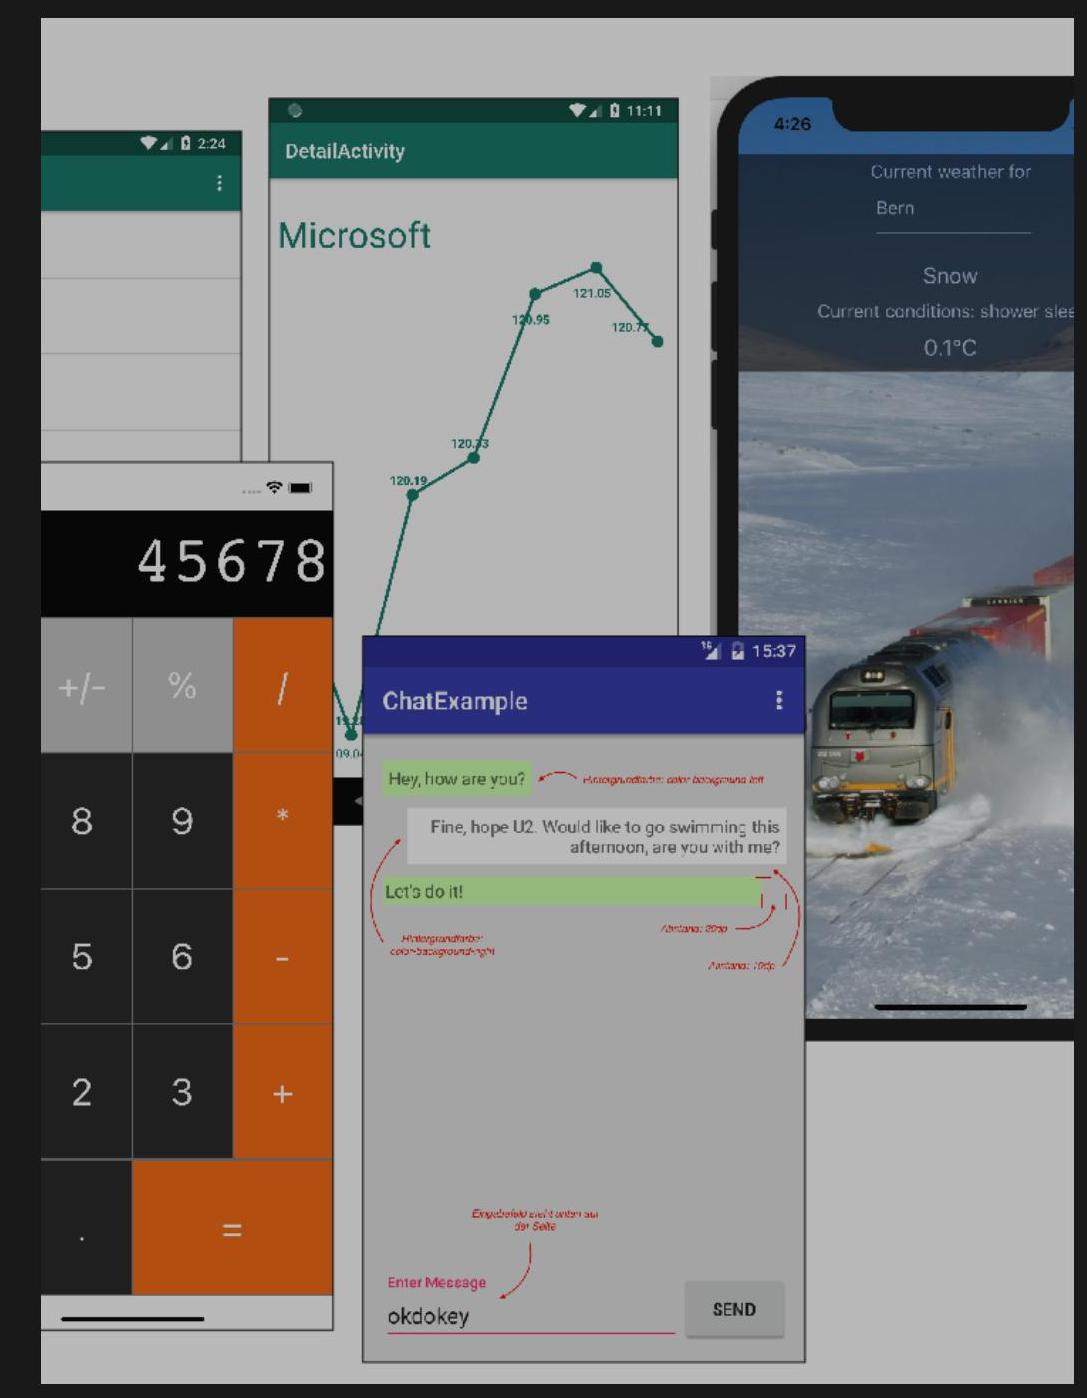
\includegraphics[width=\linewidth]{images/2025_01_02_68113d8fd21152cab1dbg-21}

\section*{Apps mit Webtechnologien}
\begin{itemize}
  \item Desktop-Applikationen mit Web-Technologien \href{https://www.electronjs.org}{https://www.electronjs.org} \href{https://nwjs.io}{https://nwjs.io}
  \item Basis für Applikationen wie VSCode
  \item Diverse weitere Frameworks in diesem Bereich
  \item Mobil-Applikationen mit Web-Technologien \href{https://cordova.apache.org}{https://cordova.apache.org} \href{https://capacitorjs.com}{https://capacitorjs.com}
\end{itemize}

\section*{WebAssembly (WASM)}
\begin{itemize}
  \item Bytecode zur Ausführung in Webbrowsern
  \item Ziel: höhere Performanz für Web-Applikationen
  \item Verschiedene Programmiersprachen kompilieren zu WASM
  \item Erste Version funktioniert in aktuellen Browsern bereits\\
\href{https://webassembly.org}{https://webassembly.org}\\
$\triangleright$ PSPP
\end{itemize}

\section*{JavaScript-Alternativen}
\begin{itemize}
  \item Werden nach JavaScript „kompiliert"
  \item TypeScript (Microsoft)
  \item statisches Typenkonzept
  \item ReScript (ehemals ReasonML)
  \item speziell für React-Ansatz geeignet
  \item funktionaler Ansatz, an OCaml angelehnt
  \item ClojureScript (Lisp-Dialekt)
  \item PSPP
\end{itemize}

\section*{Funktionale Programmierung}
\begin{itemize}
  \item JavaScript ist eine Multiparadigmensprache
  \item Es eignet sich sehr gut für funktionale Programmierung (higher order functions, partial application, currying, ...)
  \item In WBE wird dieser Aspekt kaum thematisiert
  \item PSPP\\
$\triangleright$ FUP
\end{itemize}

\section*{Programmiersprachen und -Paradigmen (PSPP)}
\begin{itemize}
  \item Compiler, Bytecodes (WASM)
  \item Logische Programmierung (Prolog)
  \item Objektorientierte Programmierung (Smalltalk)
  \item Funktionale Programmierung (Lisp, Python)
  \item und: Modulkonzept, Scriptsprachen, Typenkonzepte
\end{itemize}

Info $\triangleright$ G. Burkert (bkrt), K. Rege (rege)



\section*{Design, Usability, ...}
\begin{itemize}
  \item Grafische Gestaltung
  \item Gestaltungsprinzipien
  \item Farbenlehre
  \item Typografie
  \item Usability
  \item Barrierefreiheit\\
$\triangleright$ Vorbereitungskurs WBE (design-usability.pdf)
\end{itemize}

\section*{Zurück zu JavaScript ...}
\section*{DOUGLAS CROCKFORD}
\section*{Autor von: JavaScript: The Good Parts}
„The idea of putting powerful functions and dynamic objects in the same language was just brilliant. That's the thing that makes JavaScript interesting."

FullStack London 2018\\
\href{https://www.youtube.com/watch?v=8oGCyfautKo}{https://www.youtube.com/watch?v=8oGCyfautKo}\\
„My advice to everybody who wants to be a better programmer is to learn more languages. A good programming language should teach you. And in my career the language which has taught me the most was JavaScript."

The Better Parts. JS Fest 2018\\
\href{https://www.youtube.com/watch?v=XFTOG895C7c}{https://www.youtube.com/watch?v=XFTOG895C7c}

\section*{ÜBERSICHT}
\begin{itemize}
  \item Von SuiWeb zu React.js
  \item Ausblick: Weitere Themen rund ums Web
  \item Abschluss, Feedback
  \item Anhang: Themenliste WBE
\end{itemize}

\section*{ÜBERBLICK WBE}
\begin{center}
\begin{tabular}{|c|l|}
\hline
Woche & Thema \\
\hline
1 & Einführung, Administratives, das Web im Überblick \\
\hline
2 & JavaScript: Grundlagen \\
\hline
3 & JavaScript: Objekte und Arrays \\
\hline
4 & JavaScript: Funktionen \\
\hline
5 & JavaScript: Prototypen von Objekten \\
\hline
6 & JavaScript: Asynchrones Programmieren \\
\hline
7 & JavaScript: Webserver \\
\hline
$8-9$ & Browser-Technologien: JavaScript im Browser \\
\hline
10 & Browser-Technologien: Client-Server-Interaktion \\
\hline
$11-13$ & Ul-Bibliothek: Komponenten, Implementierung, Einsatz \\
\hline
14 & Abschluss: React, Feedback \\
\hline
\end{tabular}
\end{center}

\section*{WBE-ZIELE}
In erster Linie:\\
Solide Kenntnisse in grundlegenden Web-Technologien, speziell JavaScript, denn dies ist die Programmiersprache des Web.

\section*{Grundlagen:}
HTML und CSS als Basistechnologien des Web muss man natürlich auch kennen, um mit Webtechnologien entwickeln zu können.

\section*{Ausserdem:}
Einen Überblick erhalten über einen für heutige Anforderungen relevanten Ausschnitt aus dem riesigen Gebiet der Web-Technologien.

\section*{ALLGEMEINE BETRACHTUNG}
\begin{itemize}
  \item Themen, welche vertieft behandelt wurden
\end{itemize}

Grösserer Block in mindestens einer Vorlesung, also nicht nur zwei bis drei Slides dazu, in der Regel auch im Praktikum thematisiert

\begin{itemize}
  \item Themen welche nebenbei behandelt wurden
\end{itemize}

Im Sinne von: das gibt's auch, sollte man kennen, wenn man sich mit Webtechnologien beschäftigt, Einarbeitung nach Bedarf

\section*{ALLGEMEINE BETRACHTUNG}
\begin{itemize}
  \item Themen, welche vertieft behandelt wurden
\end{itemize}

Mit diesen Themen sollte man sich auskennen (ein paar mehr Details im Anhang)

\begin{itemize}
  \item Themen welche nebenbei behandelt wurden
\end{itemize}

Hier sollte man wissen, worum es geht, dazu gehören ein paar wesentliche Merkmale der Technologie, des Frameworks oder der Idee, aber Details sind hier nicht das Ziel

\section*{BITTE UM FEEDBACK}
\begin{itemize}
  \item Inhalte?
  \item Stoffumfang?
  \item Praktika?
  \item Art der Durchführung?
\end{itemize}

\section*{STACKOVERFLOW SURVEY, GOOGLE TRENDS}
\begin{center}
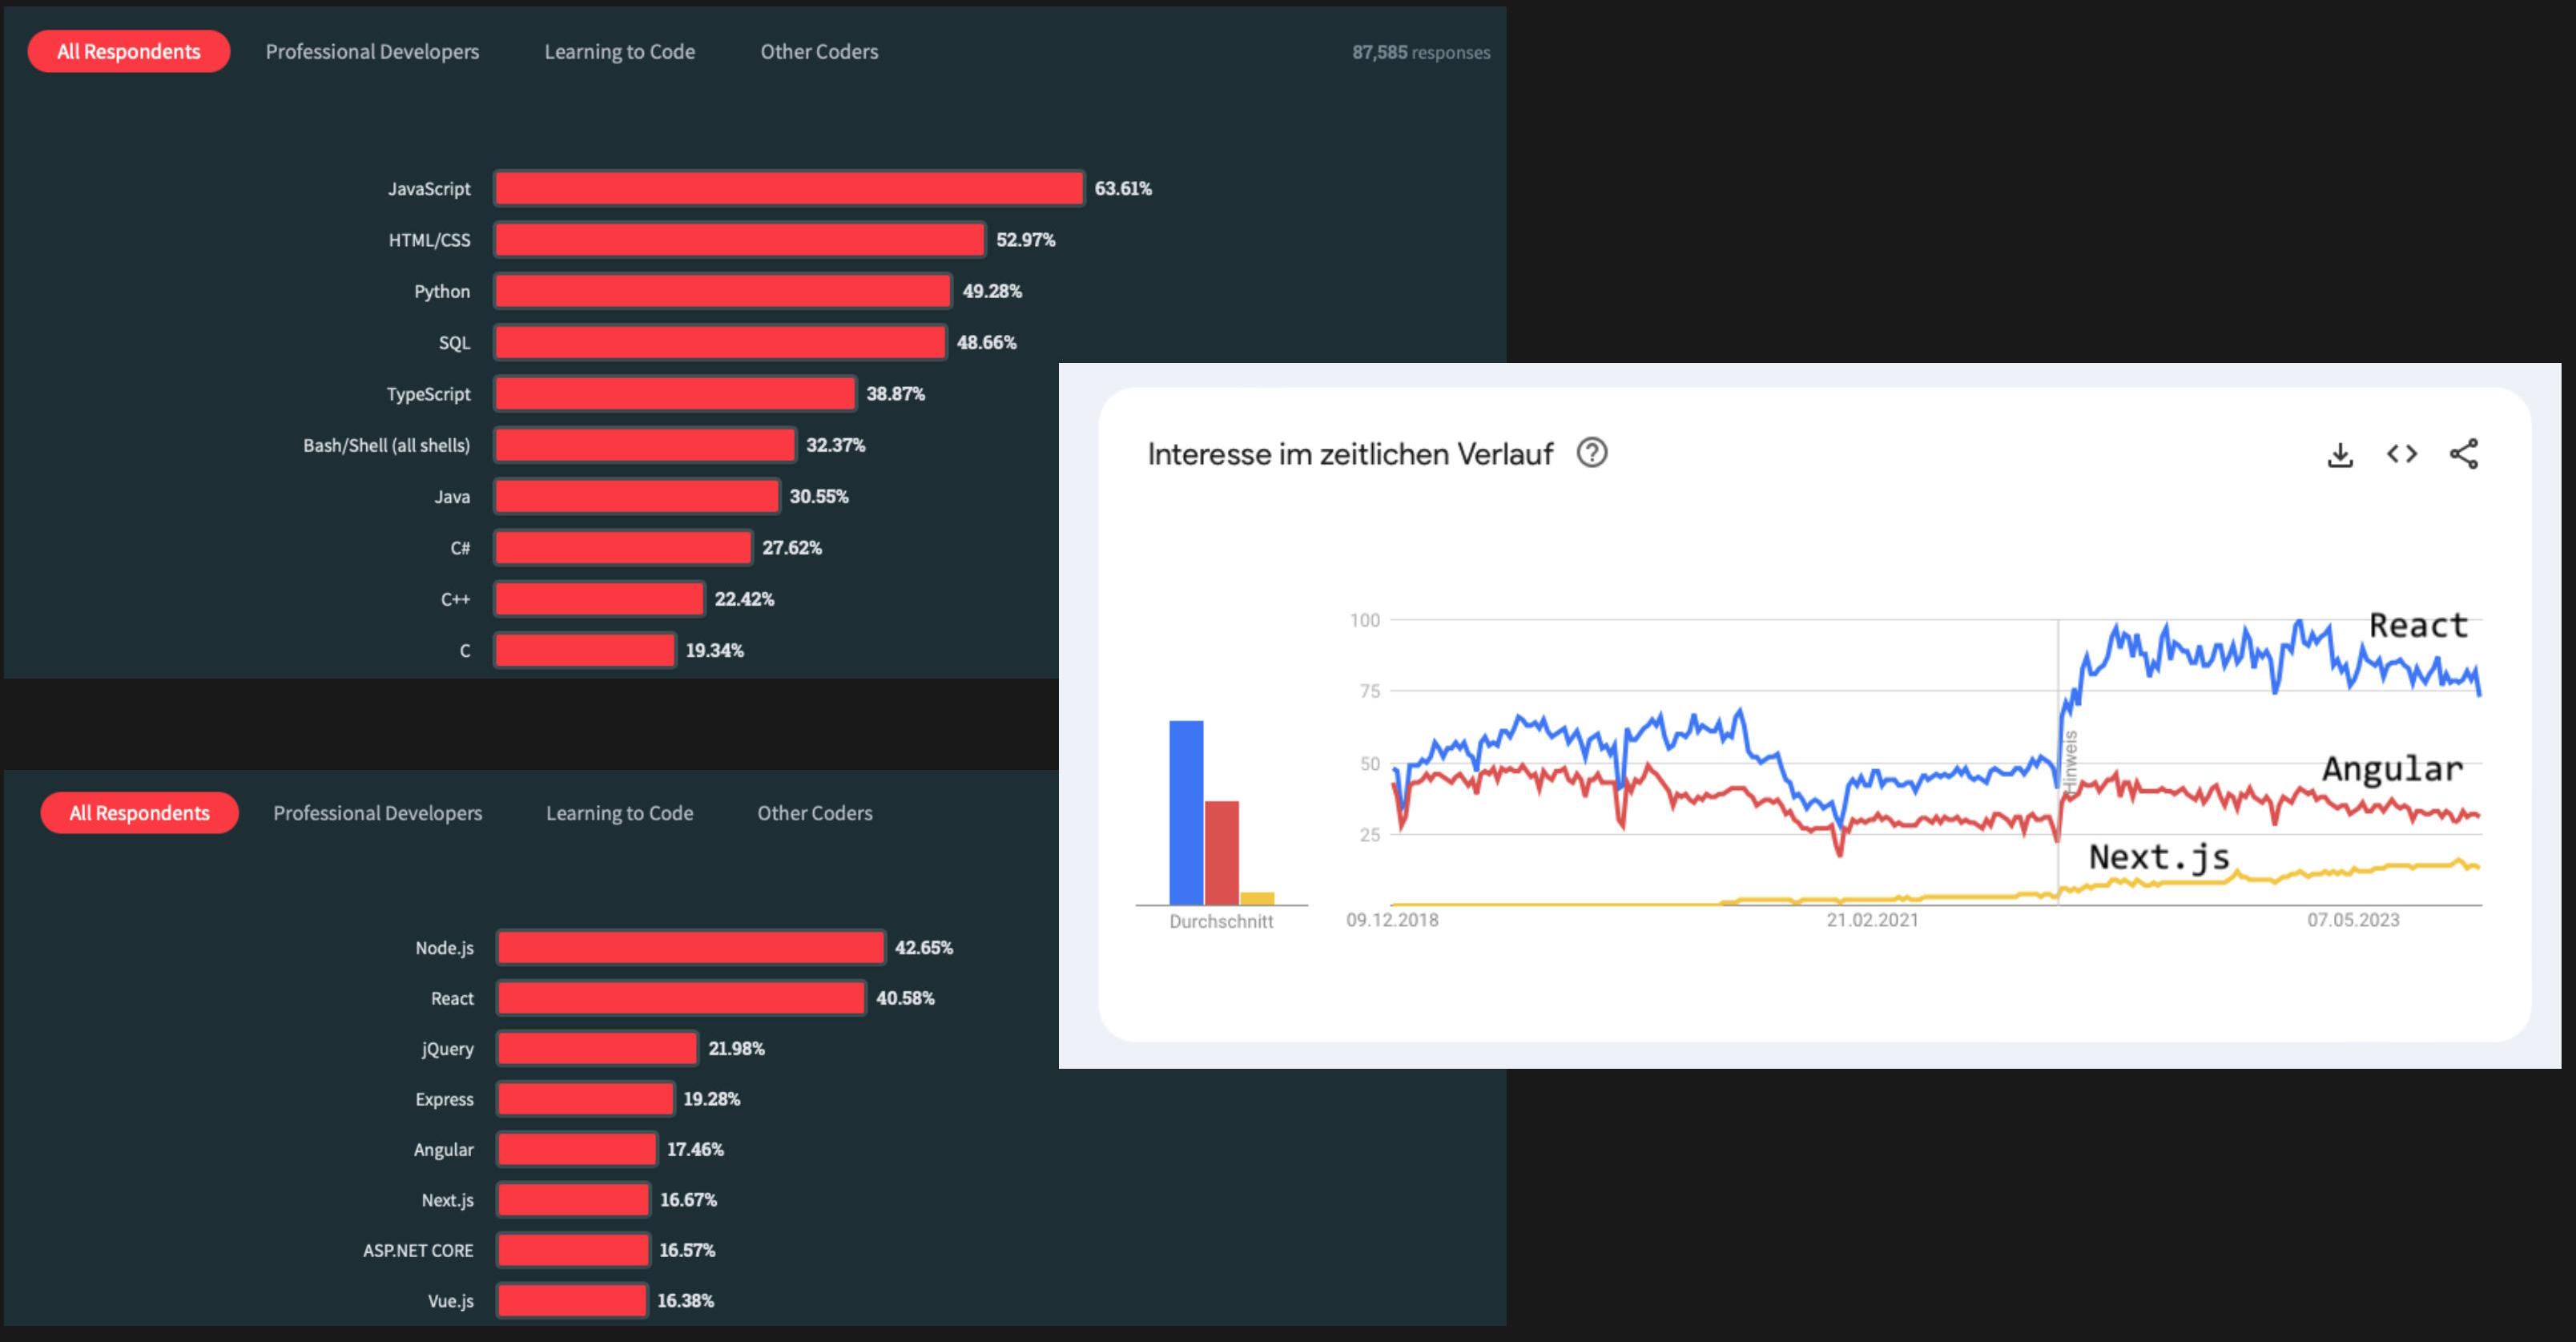
\includegraphics[width=\linewidth]{images/2025_01_02_68113d8fd21152cab1dbg-36}
\end{center}

TIOBE Index for December 2023

\begin{center}
\begin{tabular}{|c|c|c|c|c|c|c|}
\hline
Dec 2023 & Dec 2022 & Change & \multicolumn{2}{|l|}{Programming Language} & Ratings & Change \\
\hline
1 & 1 &  &  & Python & 13.86\% & -2.80\% \\
\hline
2 & 2 &  &  & C & 11.44\% & -5.12\% \\
\hline
3 & 3 &  &  & C++ & 10.01\% & -1.92\% \\
\hline
4 & 4 &  & 
\includegraphics[width=\linewidth]{images/2025_01_02_68113d8fd21152cab1dbg-37}
 & Java & 7.99\% & -3.83\% \\
\hline
5 & 5 &  &  & C\# & 7.30\% & +2.38\% \\
\hline
6 & 7 & $\wedge$ & JS & JavaScript & 2.90\% & -0.30\% \\
\hline
7 & 10 & $\wedge$ &  & PHP & 2.01\% & +0.39\% \\
\hline
15 & 23 & 入 &  & Kotlin & 0.92\% & +0.34\% \\
\hline
16 & 16 &  &  & Delphi/Object Pascal & 0.92\% & +0.07\% \\
\hline
17 & 15 & $\checkmark$ &  & Swift & 0.82\% & -0.09\% \\
\hline
18 & 20 & $\wedge$ & (19) & Rust & 0.80\% & +0.12\% \\
\hline
38 &  & cript &  &  &  &  \\
\hline
39 &  &  &  &  &  &  \\
\hline
40 &  &  &  &  &  &  \\
\hline
41 & M &  &  &  &  &  \\
\hline
\end{tabular}
\end{center}

\begin{center}

\includegraphics[width=\linewidth]{images/2025_01_02_68113d8fd21152cab1dbg-38}
\end{center}

\section*{Schöne Feiertage}
\section*{ÜBERSICHT}
\begin{itemize}
  \item Von SuiWeb zu React.js
  \item Ausblick: Weitere Themen rund ums Web
  \item Abschluss, Feedback
  \item Anhang: Themenliste WBE
\end{itemize}

\section*{ÜBERBLICK}
\begin{itemize}
  \item Ganzes Thema wichtig
  \item inklusive Unterthema
  \item Thema teilweise wichtig
  \item zum Beispiel dieses Unterthema
  \item Unterthema: Überblick genügt
  \item Überblick genügt
  \item Unterthema ebenso
\end{itemize}

\section*{GRUNDLAGEN: HTML \& CSS}
\begin{itemize}
  \item Markup und HTML
  \item Konzept von Markup verstehen
  \item Eckpunkte der Entwicklung von HTML kennen
  \item Aufbau eines HTML-Dokuments
  \item Grundbegriffe: Element, Tag, Attribut
  \item Grundlegende Elemente: html, head, title, meta, body, p, div, span, p, img, h1, ..., ul, ol, li
  \item Weitere Elemente: header, article, ...
  \item Attribute: contenteditable, data-
  \item Bild- und Grafikformate, SVG
\end{itemize}

\section*{GRUNDLAGEN: HTML \& CSS}
\begin{itemize}
  \item Darstellung mit CSS
  \item CSS mit HTML verbinden, CSS-Regeln
  \item Selektoren
  \item Einige Eigenschaften, Grössen- und Farbangaben (am besten an Beispielen und Aufgaben orientieren)
  \item Schriften laden, Transitionen, Transformationen, Animationen
  \item Weitere Eigenschaften
  \item Werkzeuge und Hilfsmittel
\end{itemize}

\section*{GRUNDLAGEN: HTML \& CSS}
\begin{itemize}
  \item Das Box-Modell
  \item overflow, width, height, margin, padding, border
  \item border-radius, color, background-color
  \item Farbverläufe, Sprites
  \item Positionierung und fliessende Boxen
  \item position, float, clear, display (block, inline, none)
\end{itemize}

\section*{1. DAS WEB}
\begin{itemize}
  \item Internet und WWW
  \item Einige Eckpunkte der Entwicklung kennen
  \item Client-Server-Architektur
  \item Konzepte und wesentliche Tools kennen
  \item User Agents, Webserver
  \item URI/URL, IP-Adresse, Domain-Name
  \item Grundzüge des HTTP-Protokolls
\end{itemize}

\section*{1. DAS WEB}
\begin{itemize}
  \item Die Sprachen des Web: HTML, CSS, JavaScript
  \item Vorkenntnisse / Vorkurs
  \item Web-Standards und APIs
  \item W3C und WHATWG kennen
  \item clientseitige vs. serverseitige Technologien
\end{itemize}

\section*{2. JAVASCRIPT GRUNDLAGEN}
\begin{itemize}
  \item JavaScript und Node.js
  \item Einige Eckpunkte der Entwicklung
  \item Node.js als JavaScript-Laufzeitumgebung
  \item Node.js Einsatz, REPL, NPM
  \item console.log
  \item Werte, Typen, und Operatoren
  \item Zahlen, typeof, Strings, logische Ausdrücke, ...
\end{itemize}

\section*{2. JAVASCRIPT GRUNDLAGEN}
\begin{itemize}
  \item Programmstruktur
  \item Ausdruck vs. Anweisung
  \item Syntax, Variablen, Kontrollstrukturen, Kommentare, ...
  \item Funktionen
  \item Überblick, mehr später
\end{itemize}

\section*{3. JS: OBJEKTE UND ARRAYS}
\begin{itemize}
  \item Objekte
  \item Objektliterale, Attribute, Methoden, ...
  \item Methoden von Object: assign, keys, values
  \item Spezielle Objekte: Arrays
  \item Array-Literale
  \item Schleifen über Arrays
  \item Array-Methoden: slice, concat, Array.isArray
  \item Weitere Methoden schaut man bei Bedarf nach
\end{itemize}

\section*{3. JS: OBJEKTE UND ARRAYS}
\begin{itemize}
  \item Werte- und Referenztypen
  \item Unterschied verstehen
  \item Wissen, welche Typen in JS Werte- und Referenztypen sind
  \item Vordefinierte Objekte, JSON
  \item Wichtigste vordefinierte Objekte kennen
  \item Methoden schaut man bei Bedarf nach
  \item JSON.stringify, JSON.parse
\end{itemize}

Zum vorletzten Punkt: Unterschied zwischen in eigenem Code verwenden und in bestehendem Code verstehen. Was ein "Hello World".indexOf("Il") bedeutet, sollte man sich schon vorstellen können.

\section*{4. JS: FUNKTIONEN}
\begin{itemize}
  \item Funktionen definieren
  \item Definition und Deklaration, Pfeilnotation
  \item Gültigkeitsbereiche
  \item Parameter von Funktionen
  \item Default-, Rest-Parameter, arguments
  \item Spread-Operator
  \item Arrays und Objekte destrukturieren
  \item Funktionen höherer Ordnung
  \item Arrays: forEach, filter, map, reduce
\end{itemize}

\section*{4. JS: FUNKTIONEN}
\begin{itemize}
  \item Closures
  \item Einsatz von Closures
  \item Pure Funktionen
  \item Funktionen dekorieren
  \item Funktionales Programmieren
  \item Mehr zu Node.js
  \item Konsole, Kommandozeilenargumente
  \item Module in JavaScript
  \item NPM, NPX
\end{itemize}

\section*{5. JS: PROTOTYPEN VON OBJEKTEN}
\begin{itemize}
  \item Prototypen und this
  \item Bedeutung von this je nach Aufruf
  \item Strict Mode
  \item call, apply, bind
  \item Prototyp eines Objekts, Object. create
  \item Weitere Methoden (getPrototypeOf, getOwnPropertyNames) schlägt man bei Bedarf nach
\end{itemize}

\section*{5. JS: PROTOTYPEN VON OBJEKTEN}
\begin{itemize}
  \item Konstruktoren und Vererbung
  \item Konstruktorfunktionen, new
  \item Prototypenkette
  \item Gewohntere Syntax: Klassen
  \item class, extends, constructor,...
  \item Test-Driven Development
  \item Konzept verstehen
  \item Jasmine einsetzen können
\end{itemize}

\section*{6. JS: ASYNCHRONES PROGRAMMIEREN}
\begin{itemize}
  \item File API
  \item Unterschied zwischen fs.readFileSync und fs.readFile
  \item Streams und weitere Methoden
  \item Reagieren auf Ereignisse
  \item Event Loop im Überblick
  \item Modul „events"
  \item Promises, Async/Await
\end{itemize}

\section*{7. JS: WEBSERVER}
\begin{itemize}
  \item Internet-Protokolle
  \item Internet-Protokoll-Stack
  \item Protokolle: FTP, SFTP, SSH
  \item Das HTTP-Protokoll
  \item Grundlagen des Protokolls
  \item HTTP-Methoden: GET, POST, PUT, PATCH, DELETE
\end{itemize}

\section*{7. JS: WEBSERVER}
\begin{itemize}
  \item Node.js Webserver
  \item Web-Server, -Client, Streams: Code lesen können
  \item Beispiel File-Server: Aufbau grob verstehen
  \item REST APIs
  \item Konzept verstehen
  \item Alternative GraphQL
  \item Express.js
  \item Für einfache Aufgaben verwenden können
  \item Reverse Proxy
\end{itemize}

\section*{8. BROWSER: JAVASCRIPT}
\begin{itemize}
  \item JavaScript im Browser
  \item Überblick, ES-Module
  \item Document Object Model
  \item Repräsentation im Speicher, Baumstruktur
  \item Verschiedene Knotentypen, Knoten anlegen
  \item Array-ähnliche Objekte, Array.from
  \item Attribute: HTML-Attribute, className, classList, style
  \item requestAnimationFrame
  \item Überblick, was möglich ist (Details kann man nachschlagen)
  \item DOM-Scripting-Code lesen können
\end{itemize}

\section*{8. BROWSER: JAVASCRIPT}
\begin{itemize}
  \item Vordefinierte Objekte
  \item Allgemeine Objekte und Browser-Objekte
  \item CSS und das DOM
  \item Layout-Angaben im DOM
  \item class und style
\end{itemize}

\section*{9. BROWSER: JAVASCRIPT}
\begin{itemize}
  \item Event Handling im Browser
  \item Events registrieren: window .addEventListener
  \item Event-Handler und Event-Objekt
  \item Event-Weiterleitung und Default-Verhalten
  \item Events: click, weitere Events
  \item Kleiner Exkurs: jQuery
  \item Bilder und Grafiken
  \item Weitere Browser-APIs
  \item WebStorage
  \item History, Geolocation, Workers
\end{itemize}

\section*{10. BROWSER: CLIENT-SERVER}
\begin{itemize}
  \item Formulare
  \item Element form mit Attributen method, action
  \item Elemente input, label mit wichtigen Attributen
  \item Mehr kann man bei Bedarf nachschlagen
  \item Daten mit GET und POST übertragen
  \item File-Input, GET und POST in Express
  \item Cookies, Sessions
  \item Konzept verstanden
\end{itemize}

\section*{10. BROWSER: CLIENT-SERVER}
\begin{itemize}
  \item Ajax und XMLHttpRequest
  \item Konzept verstanden
  \item Fetch API
  \item Verwenden von fetch (Promise)
  \item jQuery, Axios, CORS
\end{itemize}

\section*{11. UI-BIBLIOTHEK (1)}
\begin{itemize}
  \item Frameworks und Bibliotheken
  \item Unterschied, Eckpunkte der Entwicklung
  \item Model-View-Controller, Singe-Page Apps
  \item DOM-Scripting und Abstraktionen
  \item Verschiedene Ansätze im Überblick
  \item JSX und SJDON
  \item Vergleich der Notationen
  \item Eigene Bibliothek: SuiWeb
  \item Ziel, Vorgehen
\end{itemize}

\section*{12. UI-BIBLIOTHEK (2)}
\begin{itemize}
  \item Erste Schritte
  \item Interne Datenstruktur, createElement, render
  \item Ansatz verstehen, Code lesen können
  \item Komponenten und Properties
  \item Einsetzen können
  \item Details wie sie implementiert sind weniger wichtig
  \item Darstellung von Komponenten
  \item Defaults und weitere Beispiele
\end{itemize}

\section*{13. UI-BIBLIOTHEK (3)}
\begin{itemize}
  \item Zustand von Komponenten
  \item State-Hook, einsetzen können
  \item Kontrollierte Eingabe
  \item Details der Implementierung sind weniger wichtig
  \item Komponenten-Design
  \item Container-Componente
  \item Lifecycle-Methoden, Effect-Hook
  \item Aufteilen in Komponenten:
\end{itemize}

Beispiel nachvollziehen können

\begin{itemize}
  \item Deklarativer vs. imperativer Ansatz
\end{itemize}

\section*{13. UI-BIBLIOTHEK (3)}
\begin{itemize}
  \item Ausblick: Optimierungsansätze
  \item Aufteilen in Arbeitsschritte, asynchrones Abarbeiten
  \item Render- und Commit-Phasen
\end{itemize}

\section*{14. ABSCHLUSS}
\begin{itemize}
  \item Von SuiWeb zu React.js
  \item Klassenkomponenten
  \item Weitere Konzepte
  \item Ausblick: Weitere Themen rund ums Web
\end{itemize}